\documentclass[11pt,compress,t,notes=noshow, xcolor=table]{beamer}
\usepackage[]{graphicx}\usepackage[]{color}
% maxwidth is the original width if it is less than linewidth
% otherwise use linewidth (to make sure the graphics do not exceed the margin)
\makeatletter
\def\maxwidth{ %
  \ifdim\Gin@nat@width>\linewidth
    \linewidth
  \else
    \Gin@nat@width
  \fi
}
\makeatother

\newcommand{\citebutton}[2]{%
\beamergotobutton{\href{#2}{#1}}%
}

\newcommand{\blu}[1]{\textcolor{blue}{#1}}
\newcommand{\org}[1]{\textcolor{orange}{#1}}
\newcommand{\ques}{\textbf{\textcolor{red}{Question:  }}}
\newcommand{\questionssofar}{\begin{frame}\frametitle{Any questions?}\end{frame}}

\newcommand\warning{%
 \makebox[1.4em][c]{%
 \makebox[0pt][c]{\raisebox{.1em}{\scriptsize!}}%
 \makebox[0pt][c]{\color{red}\normalsize$\bigtriangleup$}}}%

\definecolor{fgcolor}{rgb}{0.345, 0.345, 0.345}
\newcommand{\hlnum}[1]{\textcolor[rgb]{0.686,0.059,0.569}{#1}}%
\newcommand{\hlstr}[1]{\textcolor[rgb]{0.192,0.494,0.8}{#1}}%
\newcommand{\hlcom}[1]{\textcolor[rgb]{0.678,0.584,0.686}{\textit{#1}}}%
\newcommand{\hlopt}[1]{\textcolor[rgb]{0,0,0}{#1}}%
\newcommand{\hlstd}[1]{\textcolor[rgb]{0.345,0.345,0.345}{#1}}%
\newcommand{\hlkwa}[1]{\textcolor[rgb]{0.161,0.373,0.58}{\textbf{#1}}}%
\newcommand{\hlkwb}[1]{\textcolor[rgb]{0.69,0.353,0.396}{#1}}%
\newcommand{\hlkwc}[1]{\textcolor[rgb]{0.333,0.667,0.333}{#1}}%
\newcommand{\hlkwd}[1]{\textcolor[rgb]{0.737,0.353,0.396}{\textbf{#1}}}%
\let\hlipl\hlkwb

\usepackage{framed}
\makeatletter
\newenvironment{kframe}{%
 \def\at@end@of@kframe{}%
 \ifinner\ifhmode%
  \def\at@end@of@kframe{\end{minipage}}%
  \begin{minipage}{\columnwidth}%
 \fi\fi%
 \def\FrameCommand##1{\hskip\@totalleftmargin \hskip-\fboxsep
 \colorbox{shadecolor}{##1}\hskip-\fboxsep
     % There is no \\@totalrightmargin, so:
     \hskip-\linewidth \hskip-\@totalleftmargin \hskip\columnwidth}%
 \MakeFramed {\advance\hsize-\width
   \@totalleftmargin\z@ \linewidth\hsize
   \@setminipage}}%
 {\par\unskip\endMakeFramed%
 \at@end@of@kframe}
\makeatother

\definecolor{shadecolor}{rgb}{.97, .97, .97}
\definecolor{messagecolor}{rgb}{0, 0, 0}
\definecolor{warningcolor}{rgb}{1, 0, 1}
\definecolor{errorcolor}{rgb}{1, 0, 0}
\newenvironment{knitrout}{}{} % an empty environment to be redefined in TeX

\usepackage{alltt}
\newcommand{\SweaveOpts}[1]{}  % do not interfere with LaTeX
\newcommand{\SweaveInput}[1]{} % because they are not real TeX commands
\newcommand{\Sexpr}[1]{}       % will only be parsed by R
\newcommand{\xmark}{\ding{55}}%


\usepackage[english]{babel}
\usepackage[utf8]{inputenc}

\usepackage{dsfont}
\usepackage{verbatim}
\usepackage{amsmath}
\usepackage{amsfonts}
\usepackage{amssymb}
\usepackage{bm}
\usepackage{csquotes}
\usepackage{multirow}
\usepackage{longtable}
\usepackage{booktabs}
\usepackage{enumerate}
\usepackage[absolute,overlay]{textpos}
\usepackage{psfrag}
\usepackage{algorithm}
\usepackage{algpseudocode}
\usepackage{eqnarray}
\usepackage{arydshln}
\usepackage{tabularx}
\usepackage{placeins}
\usepackage{tikz}
\usepackage{setspace}
\usepackage{colortbl}
\usepackage{mathtools}
\usepackage{wrapfig}
\usepackage{bm}
\usepackage{amsmath}
\usepackage{pifont}

\usetikzlibrary{shapes.multipart,shapes,arrows,automata,positioning,calc,chains,trees, shadows}
\tikzset{
  %Define standard arrow tip
  >=stealth',
  %Define style for boxes
  punkt/.style={
    rectangle,
    rounded corners,
    draw=black, very thick,
    text width=6.5em,
    minimum height=2em,
    text centered},
  % Define arrow style
  pil/.style={
    ->,
    thick,
    shorten <=2pt,
    shorten >=2pt,}
}

\tikzstyle{vec}=[draw, rectangle, fill = white, minimum width=5mm, minimum height=1cm, inner sep = 2pt]

\usepackage{subfig}

% Defines macros and environments
\usepackage{../../style/lmu-lecture}


\let\code=\texttt
\let\proglang=\textsf

\setkeys{Gin}{width=0.9\textwidth}

\setbeamertemplate{frametitle}{\expandafter\uppercase\expandafter\insertframetitle}

\usepackage{bbm}
% basic latex stuff
\newcommand{\pkg}[1]{{\fontseries{b}\selectfont #1}} %fontstyle for R packages
\newcommand{\lz}{\vspace{0.5cm}} %vertical space
\newcommand{\dlz}{\vspace{1cm}} %double vertical space
\newcommand{\oneliner}[1] % Oneliner for important statements
{\begin{block}{}\begin{center}\begin{Large}#1\end{Large}\end{center}\end{block}}


%new environments
\newenvironment{vbframe}  %frame with breaks and verbatim
{
 \begin{frame}[containsverbatim,allowframebreaks]
}
{
\end{frame}
}

\newenvironment{vframe}  %frame with verbatim without breaks (to avoid numbering one slided frames)
{
 \begin{frame}[containsverbatim]
}
{
\end{frame}
}

\newenvironment{blocki}[1]   % itemize block
{
 \begin{block}{#1}\begin{itemize}
}
{
\end{itemize}\end{block}
}

\newenvironment{fragileframe}[2]{  %fragile frame with framebreaks
\begin{frame}[allowframebreaks, fragile, environment = fragileframe]
\frametitle{#1}
#2}
{\end{frame}}


\newcommand{\myframe}[2]{  %short for frame with framebreaks
\begin{frame}[allowframebreaks]
\frametitle{#1}
#2
\end{frame}}

\newcommand{\remark}[1]{
  \textbf{Remark:} #1
}


\newenvironment{deleteframe}
{
\begingroup
\usebackgroundtemplate{
\includegraphics[width=\paperwidth,height=\paperheight]{../style/color/red.png}}
 \begin{frame}
}
{
\end{frame}
\endgroup
}
\newenvironment{simplifyframe}
{
\begingroup
\usebackgroundtemplate{
\includegraphics[width=\paperwidth,height=\paperheight]{../style/color/yellow.png}}
 \begin{frame}
}
{
\end{frame}
\endgroup
}\newenvironment{draftframe}
{
\begingroup
\usebackgroundtemplate{
\includegraphics[width=\paperwidth,height=\paperheight]{../style/color/green.jpg}}
 \begin{frame}
}
{
\end{frame}
\endgroup
}
% https://tex.stackexchange.com/a/261480: textcolor that works in mathmode
\makeatletter
\renewcommand*{\@textcolor}[3]{%
  \protect\leavevmode
  \begingroup
    \color#1{#2}#3%
  \endgroup
}
\makeatother





\input{../../latex-math/basic-math.tex}
\input{../../latex-math/basic-ml.tex}

\newcommand{\titlefigure}{figure/sesamestreet.jpeg}
\newcommand{\learninggoals}{
\item Replaced Token Detection task
\item Interplay of Generator and Discriminator}

\title{Using the Transformer}
% \author{}
\institute{\href{https://slds-lmu.github.io/lecture_dl4nlp/}{slds-lmu.github.io/lecture\_dl4nlp}}
\date{}

\begin{document}
\lecturechapter{ELECTRA (Clark et al., 2019)}
\lecture{Deep Learning for NLP}

% ------------------------------------------------------------------------------

\begin{frame}{ELECTRA \href{https://arxiv.org/pdf/2003.10555.pdf}{\beamergotobutton{Clark et al. (2020)}}}

	\textbf{ELECTRA: a different pre-training objective}

	\begin{itemize}
		\item (Small) generator model $G$ + (large) Discriminator model $D$
		\item Generator task: Masked language modeling
		\item Discriminator task: \textit{Replaced token detection}
		\item ELECTRA learns from \textit{all} of the tokens (not just from a small portion, like e.g. BERT)
	\end{itemize}
	
	\begin{figure}
		\centering
		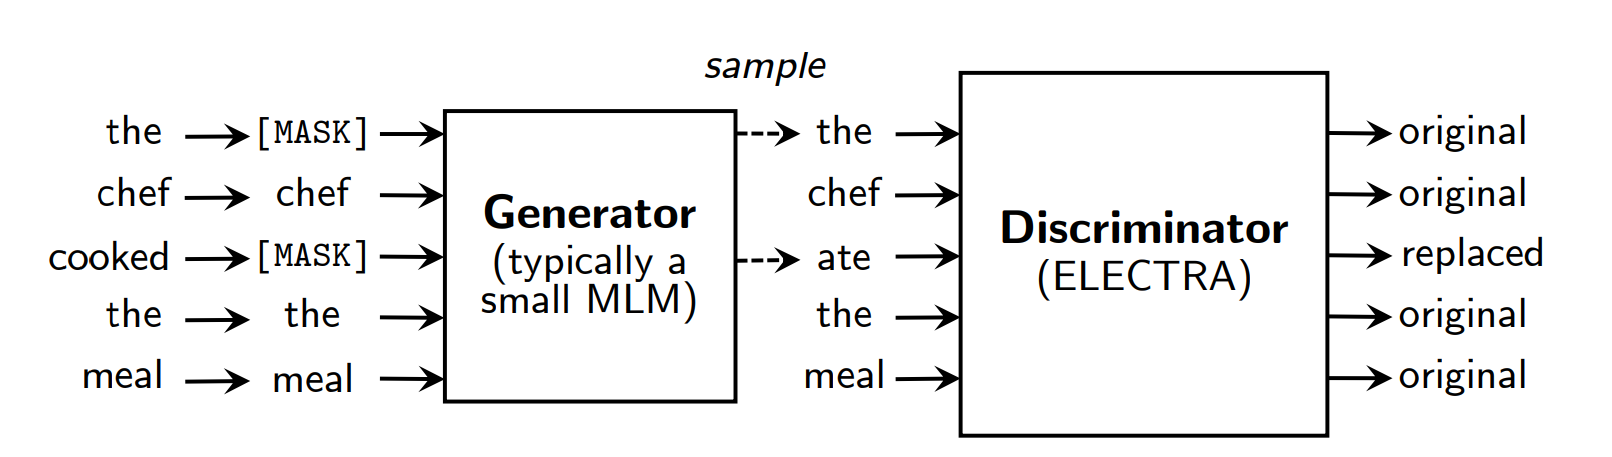
\includegraphics[width = 11cm]{figure/electra.png}\\ 
		\footnotesize{Source:} \href{https://arxiv.org/pdf/2003.10555.pdf}{\footnotesize Clark et al. (2020)}
	\end{figure}
\end{frame}

% ------------------------------------------------------------------------------

\begin{frame}{ELECTRA -- Training details}
	\textbf{Joint pre-training (but \textbf{not} in a GAN-fashion):}

	\begin{itemize}
		\item $G$ and $D$ are (Transformer) encoders which are trained jointly
		\item $G$ replaces \texttt{[MASK]}s in an input sequence\\
					$\rightarrow$ Passes corrupted input sequence $\vec{x}^{corrupt}$ to $D$
		\item \textit{Generation of samples:}
	\begin{figure}
		\centering
		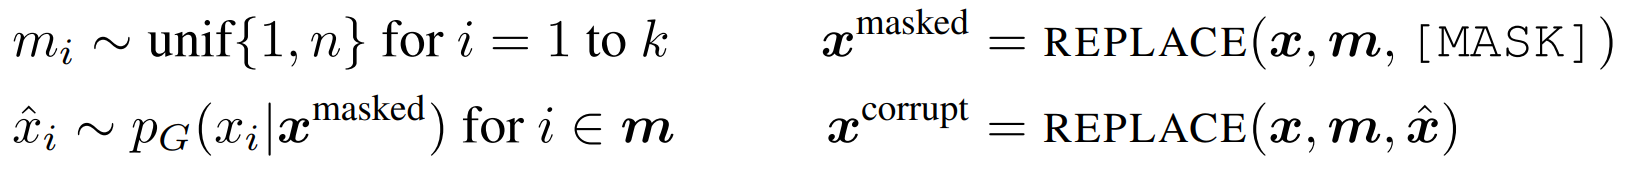
\includegraphics[width = 11cm]{figure/electra-samples.png}
	\end{figure}\vspace{-.25cm}
		{\footnotesize with approx. 15\% of the tokens masked out (via choice of $k$)}
		\item $D$ predicts whether $x_t,\; t \in 1, \hdots, T$ is "\textit{real}" or generated by $G$
			\begin{itemize}
				\item Softmax output layer for $G$ (probability distr. over all words)
				\item Sigmoid output layer for $D$ (Binary classification real vs. generated)
			\end{itemize}
	\end{itemize}
\end{frame}

% ------------------------------------------------------------------------------

\begin{frame}{ELECTRA -- Training details}

	Using the masked \& corrupted input sequences, the (joint) loss can be written down as follows:\\
	\vspace{.3cm}
	\textbf{Loss functions:}
	\begin{figure}
		\centering
		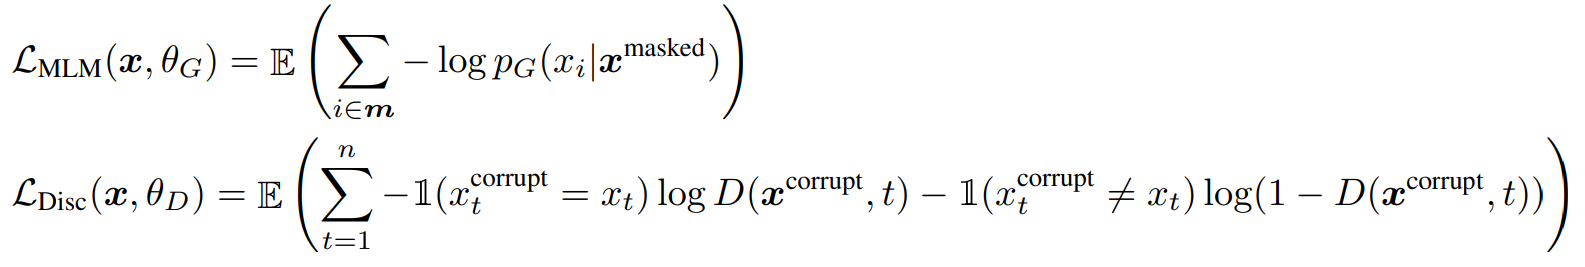
\includegraphics[width = 11cm]{figure/electra-loss.png}
	\end{figure}
	
	\textbf{Combined:}
	\begin{figure}
		\centering
		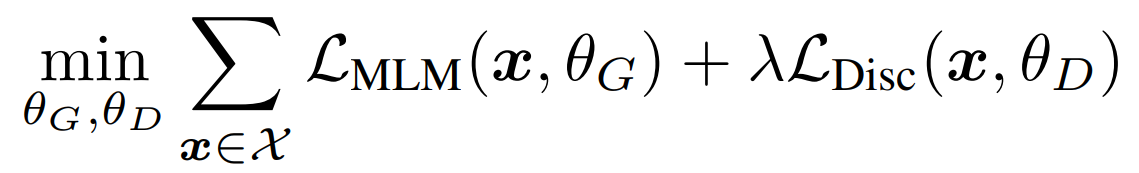
\includegraphics[width = 6cm]{figure/electra-loss-comb.png}
	\end{figure}
	{\footnotesize with $\lambda$ set to 50, since the discriminator's loss is typically much lower than the geneator's.}
\end{frame}

% ------------------------------------------------------------------------------

\begin{frame}{ELECTRA -- Training details}
\small
	\textbf{Generator size:}

	\begin{itemize}
		\item Same size of $G$ and $D$: 
			\begin{itemize}
				\item Twice as much compute per training step + too challenging for $D$
			\end{itemize}
		\item Smaller Generators are preferable (1/4 -- 1/2 the size of $D$)
	\begin{figure}
		\centering
		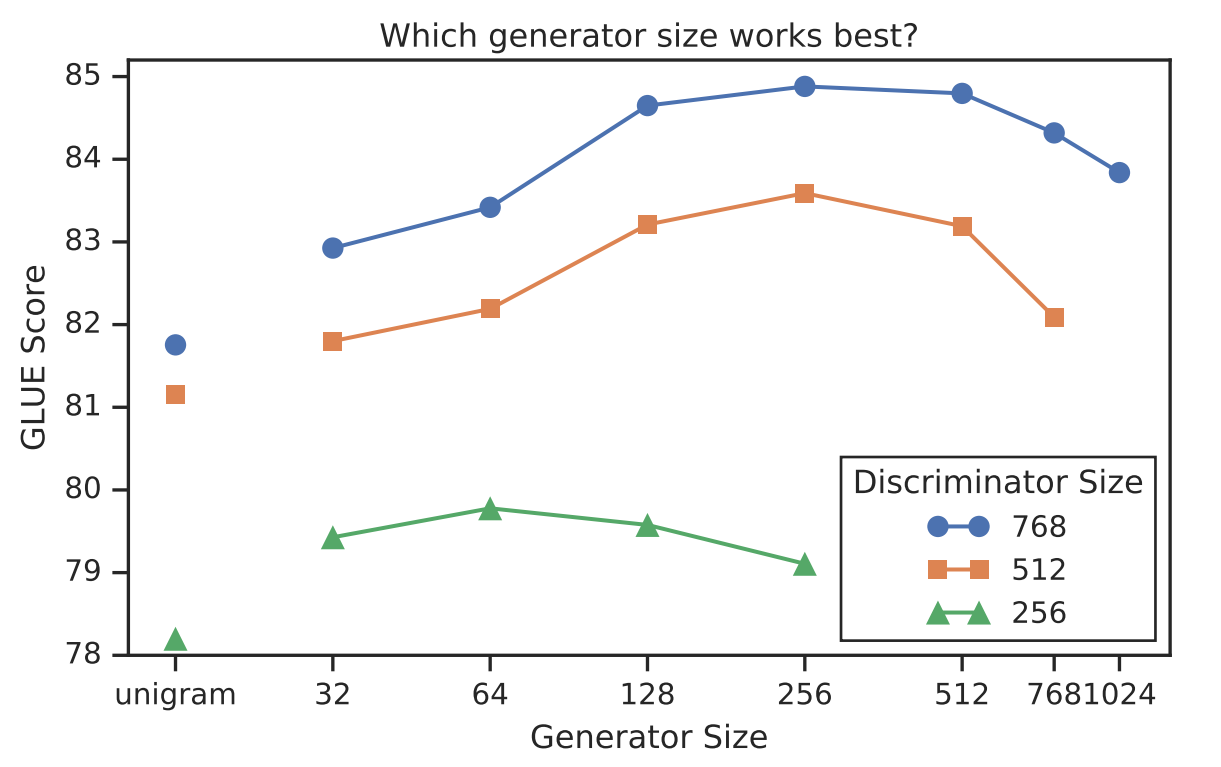
\includegraphics[width = 5cm]{figure/electra-size-g.png}\\ 
		\scriptsize{Source:} \href{https://arxiv.org/pdf/2003.10555.pdf}{\scriptsize Clark et al. (2020)}
	\end{figure}
	\end{itemize}
	
	\textbf{Weight sharing (experimental):}

	\begin{itemize}
		\item Same size of $G$ and $D$: All weights can be tied
		\item $G$ smaller than $D$: Share token \& positional embeddings 
	\end{itemize}
\end{frame}

% ------------------------------------------------------------------------------

\begin{frame}{ELECTRA -- Model comparison}
	
	\begin{figure}
		\centering
		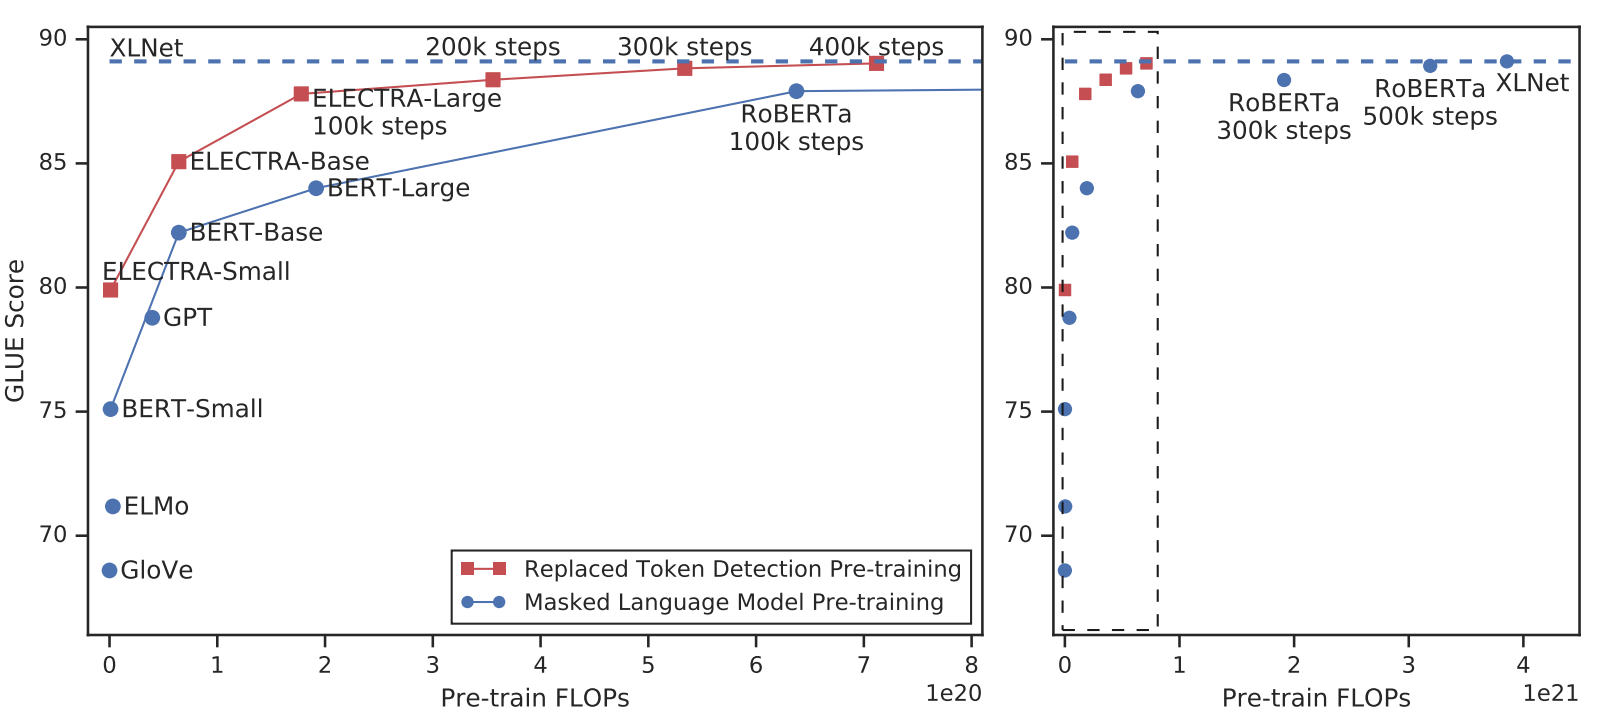
\includegraphics[width = 11cm]{figure/electra-glue.png}\\ 
		\footnotesize{Source:} \href{https://arxiv.org/pdf/2003.10555.pdf}{\footnotesize Clark et al. (2020)}
	\end{figure}
	
{\footnotesize \textit{Note:} Different batch sizes (2k vs. 8k) for ELECTRA vs. RoBERTa/XLNet explain why same number of steps lead to approx. 1/4 of the compute for ELECTRA.}
\end{frame}

% ------------------------------------------------------------------------------

\begin{frame}{ELECTRA -- SOTA performance}
\small
	\textbf{Performance differences vs. BERT/RoBERTa (GLUE dev set):}

	\begin{figure}
		\centering
		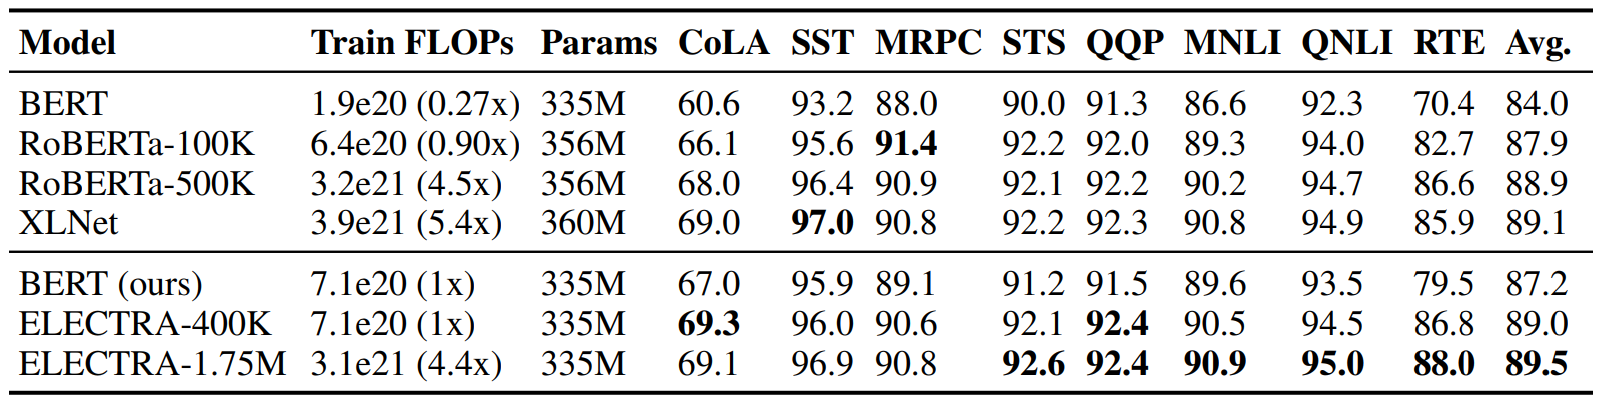
\includegraphics[width = 9cm]{figure/electra-sota1.png}\\ 
		{\footnotesize Source: \href{https://arxiv.org/pdf/2003.10555.pdf}{Clark et al. (2020)}}
	\end{figure}

	\textbf{SOTA performance (GLUE test set):}

	\begin{figure}
		\centering
		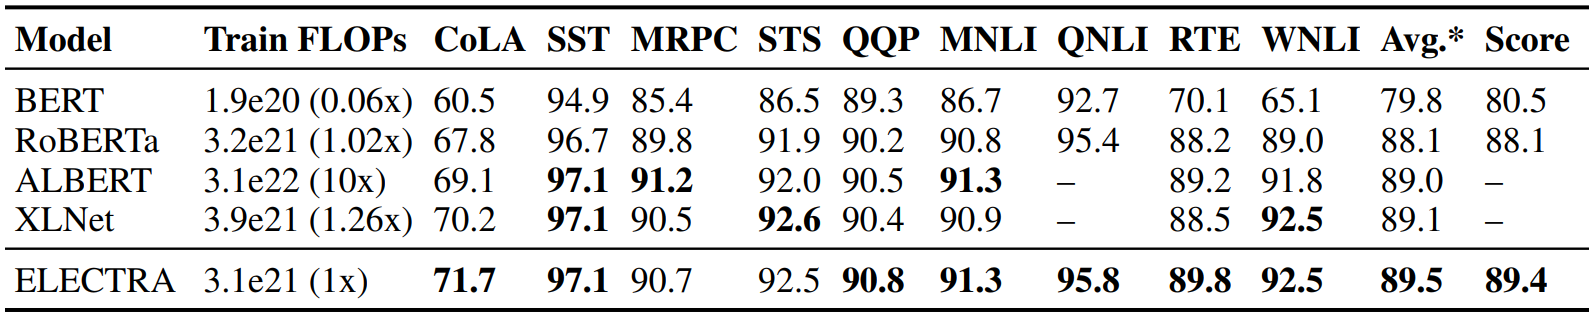
\includegraphics[width = 9cm]{figure/electra-sota2.png}\\ 
		{\tiny * Avg. excluding QNLI to ensure comparability\\\footnotesize Source: \href{https://arxiv.org/pdf/2003.10555.pdf}{Clark et al. (2020)}}
	\end{figure}
\end{frame}

% ------------------------------------------------------------------------------

\endlecture
\end{document}
